\documentclass[11pt]{beamer}
\usetheme{CambridgeUS}
\usecolortheme{orchid}

\usepackage[utf8]{inputenc}
\usepackage[brazil]{babel}
\usepackage[T1]{fontenc}

\usepackage{amsmath}
\usepackage{amsfonts}
\usepackage{amssymb}
\usepackage{graphicx}
\usepackage{setspace}
\usepackage{ragged2e}
\usepackage{gensymb}


\setbeamertemplate{caption}[numbered]
\setbeamercovered{transparent} 
\setbeamertemplate{navigation symbols}{}

\author[Joao Victor]{% 
	Joao Victor}
\title[Introdução à Geofísica Espacial]{Introdução à Geofísica Espacial}
\institute[]{% 	
	\textsuperscript{} Graduando em Licenciatura em Matemática
}
%\titlegraphic{
\includegraphics[width=0.2\textwidth]{imagens/logo_3.jpg}}
\date{\today} 
%\subject{}

% ---------------------------------------------------------

\begin{document}
\justifying
\onehalfspacing 

\begin{frame}
    \titlepage
\end{frame}

\begin{frame}{Sumário}
	\tableofcontents
\end{frame}

\section{Fotoquímica e Luminescência Atmosférica}

	\begin{frame}{Introdução}
		A atmosfera superior é uma fonte permanente de emissão de fótons que
		são liberados por átomos (moléculas) excitadas acima de seu nível normal de
		energia. A produção desta luminescência é devida a diversos processos físico-químicos e, em geral, ocorre através da emissão de linhas espectrais discretas. (pg. 53)
	\end{frame}
	
	\begin{frame}{Luminescência atmosférica}
		\begin{itemize}
			\item \textbf{airglow} é em geral muito fraca para ser visível a olho nu;
			\item \textbf{dayglow} luminescência atmosférica durante o dia, é mais difícil de ser medida, por causa da presença de luz solar direta e do espelhamento \textit{Rayleigh};
			\item \textbf{nightglow} luminescência atmosférica durante a noite. 
		\end{itemize}
	\end{frame}
	
	\begin{frame}{Luminescência - aurora}
		\begin{itemize}
			\item Predomina nas grandes latitudes e se distribui numa região de formato oval em torno de 67\degree de latitude geomagnética. é visível a olho nu;
			
			\item Durante as grandes tempestades magnéticas, as auroras são visíveis também em latitudes mais baixas;
		
		\end{itemize}
	\end{frame}
	
	\begin{frame}{Luminescência - aurora}
		\begin{itemize}
			\item Durante a atividade magnética intensa, a oval em geral se torna mais larga.
			
			\begin{center}
				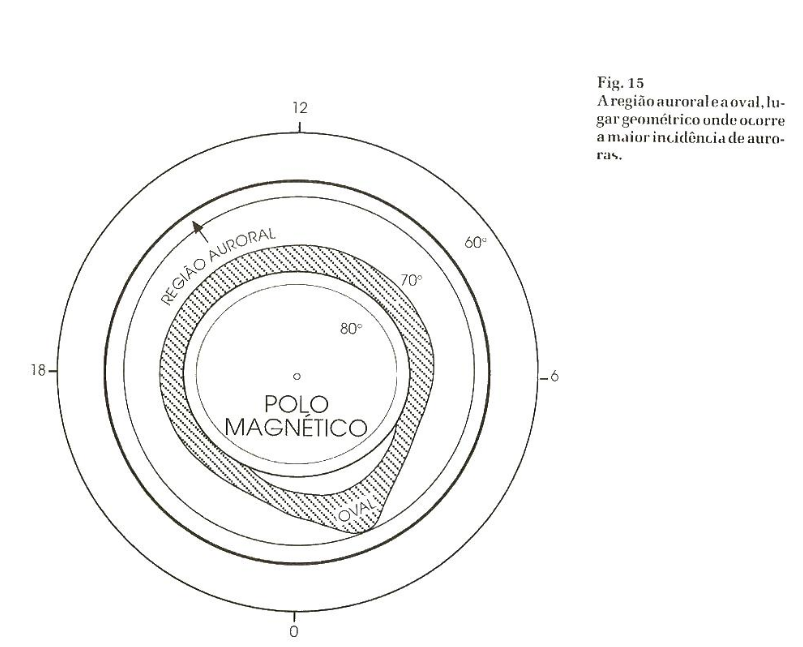
\includegraphics[scale=0.25]{imagens/aurora.png}
			\end{center}
		\end{itemize}
	\end{frame}
	
\section{Referências}
	\begin{frame}{Referências}
		\begin{itemize}
			\item Criativa EaD. (2020). O Que É O Moodle E Quais Suas Principais Características?. Disponível em  \href{https://bit.ly/amvb894hg}{Criativa EaD}
			\item Lima, José Maria Maciel. (2021) Plataforma Moodle: A educação por mediação tecnológica. Revista Científica Multidisciplinar Núcleo do Conhecimento. Ano 06, Ed. 01, Vol. 07, pp. 17-37. Disponível em: \href{https://bit.ly/9mb7b2}{<link>} 
			\item Must University. O Moodle como Plataforma de Ensino a Distância. Disponível em: \href{https://edu612tema19v2pt.webflow.io/}{Must University} 
			\item Moodle UTFPR. Disponível em: \href{https://moodle.utfpr.edu.br/login/index.php}{Moodle UTFPR Curitiba}
		\end{itemize}
	\end{frame}
\end{document}